\section{Differential cross-section}

%-------------------------
\subsection{Alignment}

\> the three methods: collimation, track-based and with physics processes

\> the new approach for alignment with elastics
\>> excellent for relative alignment (between near and far or left and right)
\>> absolute (= wrt.~the beam) achieved with the right arm and two complementary methods:

\noindent 1) standard method with vertical RPs
\noindent 2) fitting the axis of diffractive-proton axis and extrapolation to beam position

\> final uncertainty, also propagated to $\theta^*_{x, y}$ angles

\> the observed hit inefficiencies -- possible asymmetries -- discuss ???
\> mention final alignment check = 2D Gaussian fit of $\theta_x^*$ vs.~$\theta_y^*$ from both diagonals ??


%-------------------------
\subsection{Kinematics reconstruction}

\> choice of reconstruction formulae in x and in y
\>> guide = robustness against error sources: beam divergence, sensor pitch, misalignment, vertex term neglected, optics imperfections
\>> two types of reconstruction: one-arm (for cuts) and two-arm (for physics)
\>> TODO: what reco formulae used

\> typical values of uncertainties: statistical (smearing) and systematic (optics, ...)

%-------------------------
\subsection{Elastic tagging}

\> the three main cuts: left-right collinearity in $x$ and $y$, left-right vertex $x^*$ comparison
\>> motivation, sigmas
\> applied at 4 sigmas ??
\> inefficiency of the cuts (how many true events lost)

\> control cuts (not applied, used for validation only): $y^{N}$ vs.~local $\theta_y$ correlation, reconstructed $x^*$ compatible with vertex distribution?


%-------------------------
\subsection{Background}

\> background = impurity of the cuts above

\> method: plot a cut quantity under various cuts
\>> central peak (signal) stays
\>> tails (background) drop
\>> residual after all cuts $\rightarrow$ interpolate to signal region $\rightarrow$ background negligible
\>> can be repeated for any cut -- compatible results ??

\> further test: $|t|$-distributions under various combinations of cuts -- background distributed uniformly over $|t|$, no peaking

%-------------------------
\subsection{Efficiencies}

\> ``standard procedure'' for the standard contributions (ref. to previous publications?): ``3-out-of-4'' (uncorrelated 1-RP inefficiencies), ``shower in near'' (near-far correlated) and ``pile-up'' (coincidence with beam-halo or any other particle)

\> 3-out-of-4 results
\>> right arm: typical results (near $\approx 98\un{\%}$, far $\approx 96.5\un{\%}$ efficiency)
\>> left arm: efficiency in far RP unexpectedly low ($\approx 90\un{\%}$) -- due to showers in horizontal RPs (horizontal in left arm closer that in the right one) -- but experimentally determinable and thus fully correctable

\> pile-up results shown in Fig.~\ref{fig:overview}
\>> strong time-dependece: linear rise within the data-taking periods, decrease in beam cleanings


%-------------------------
\subsection{Acceptance correction}

\> ``standard procedure'' (ref. to previous publications?): ``divergence'' and ``phi'' corrections

\> also applied $-50 < \theta_x^* < 80\un{\mu rad}$ selection to avoid the regions affected by the horizontal RPs


%-------------------------
\subsection{Unfolding of resolution effects}

\> ``standard procedure'' (ref. to previous publications?)

\> but time-dependent smearing sigma, determined from the variation of $\theta_y^{*R} - \theta_y^{*L}$
\>> mention the subtlety with $\sigma(\theta_x^*)$ ?? Cannot be measured directly. The only handle comes from the emittances (crude only). But (at least for low-$|t|$), the impact of $\theta_x^*$ smearing is small -- the value of $\theta^*$ is mostly made by $\theta_y^*$, therefore $\theta_x^*$ must be very small. Consequently, $\Delta t_x = 2 \theta_x^* \Delta \theta_x^* \approx 0$

\> due to the very small beam divergence, the effect is negligible for all bins except the low-$|t|$ ones where the rapid cross-section growth appears because of the Coulomb interaction

%-------------------------
\subsection{Luminosity}

\> determined by fitting $\d N/\d t$ from $1000\un{m}$ to $\d\sigma/\d t$ from $90\un{m}$ (where the luminosity-independent method was applied, yielding $4\un{\%}$ uncertainty)

\> full uncertainty $\approx 5\un{\%}$


%-------------------------
\subsection{Systematic uncertainties}

\> ``standard procedure'' (ref. to previous publications?) of uncertainty assessment

\> leading uncertainties: residual misalignment (very low-$|t|$), normalisation (flat)

\> compatible results obtained if data right after or right before beam cleaning are used



%--------------------------------------------------
\subsection{Result}

\begin{figure*}
\begin{center}
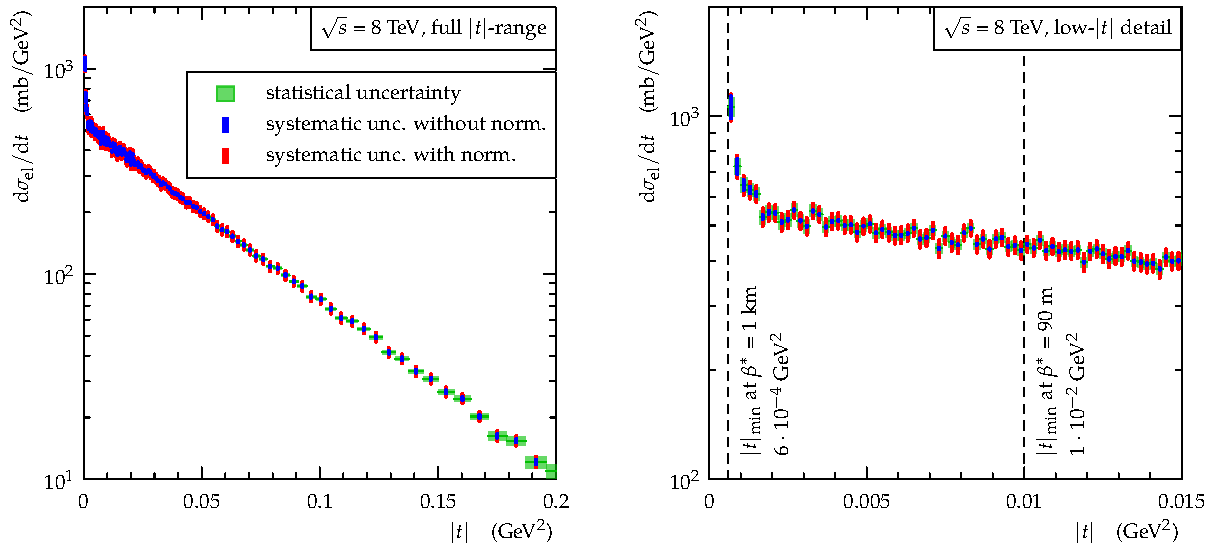
\includegraphics[width=16cm]{fig/plotTabulation.pdf}
\vskip-3mm
\caption{Differential cross-section.}
\label{fig:dsdt}
\end{center}
\end{figure*}

\> present/comment Fig.~\ref{fig:dsdt}

\> Table with points? Now or later (in a compilation with all 8 TeV data)?

